%!TEX root = ../informe.tex
\chapter{Cap\'itulo B}
\label{chap:B}

Curabitur ut nibh at mauris sagittis sagittis. Maecenas faucibus odio est, sit amet blandit nibh cursus eu. Suspendisse velit urna, mollis quis enim scelerisque, sodales imperdiet lacus. Nunc leo dui, cursus finibus accumsan non, euismod eu libero. Phasellus vitae odio ligula. Morbi lacinia, urna non tincidunt tincidunt, nibh nisi blandit lorem, eget vulputate nulla dui at augue. Sed elementum varius tortor, ut elementum sem placerat sed. Cras scelerisque urna felis, at imperdiet nulla congue ac. Nulla rhoncus elementum lorem sed suscipit. Morbi vitae consequat tellus, eget eleifend urna. Pellentesque habitant morbi tristique senectus et netus et malesuada fames ac turpis egestas. Cras ut ex ac magna egestas interdum.  

\begin{enumerate}
	\item Aliquam consequat metus ut nulla ultrices, ac lacinia dui fringilla.
	\item Mauris vestibulum ante a pharetra maximus.
	\item Sed efficitur odio ac urna mattis convallis.
	\item Nullam sodales nulla id urna convallis pulvinar.
\end{enumerate}

\section{Una secci\'on del cap\'itulo B}

Morbi quis viverra lorem, ac pulvinar ex. Cras at condimentum metus. Vestibulum turpis risus, ultricies vel ipsum id, tempor tincidunt lacus. Integer dolor est, suscipit et nisi ac, tristique facilisis lacus. Aenean consectetur dignissim luctus. Nullam eget quam dapibus, sollicitudin felis a, laoreet lorem. Nulla purus tortor, mattis id urna sagittis, porttitor auctor mi.

Nulla ut urna nibh. Aliquam et dignissim tortor. Ut ultrices risus urna, vitae convallis leo aliquet in. Ut vel nunc purus. Aliquam sagittis ex et neque venenatis, eget suscipit ipsum elementum. Phasellus eget orci ac orci vestibulum condimentum. Nullam scelerisque, orci id ultricies bibendum, nunc arcu semper nunc, vitae venenatis orci orci volutpat enim. Aliquam eget elementum nisi. Ut sed semper massa.
		
\subsection{Una subsecci\'on del cap\'itulo B}		
Neque porro quisquam est qui dolorem ipsum quia dolor sit amet, consectetur, adipisci velit:
		
\begin{equation}
	R_{1} = \frac{V_{START} - V_{STOP}}{3 \mu A} = 100K
\end{equation}
		
\begin{equation}
	R_{2} = \frac{V_{EN}}{\frac{V_{START} - V_{EN}}{R_{1}} + 1 \mu A} = 22K
\end{equation}

\begin{figure}[h]
    \centering
    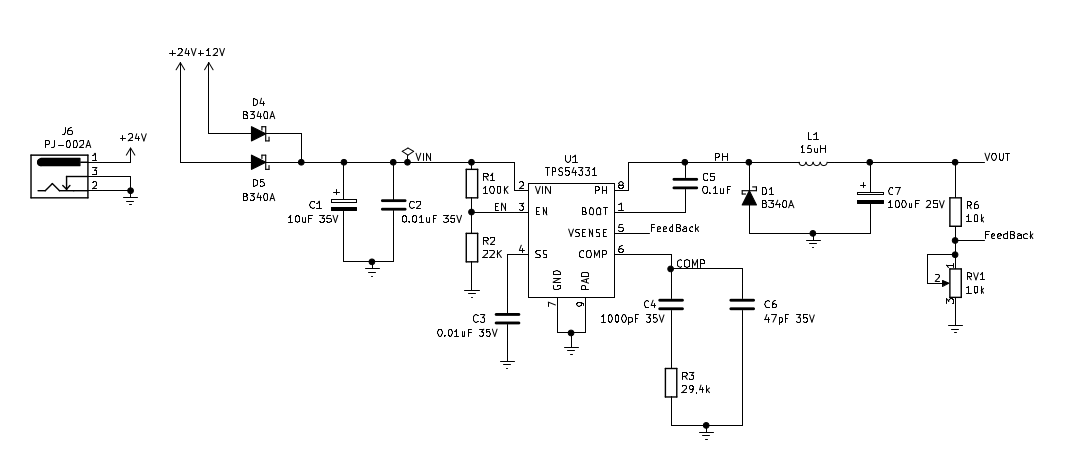
\includegraphics[width=\textwidth]{figures/chapterB/fuente.png}
    \caption{Orci id ultricies bibendum}
    \label{B_fuente}
\end{figure}

\subsection{Otra subsecci\'on del cap\'itulo B}	

Integer vitae orci eget tellus malesuada imperdiet. Cras convallis eu nisi vitae viverra. Sed nec odio tortor. Sed sed est velit. Pellentesque euismod volutpat sapien, ac malesuada mauris sollicitudin quis. Quisque id sodales nibh. Aliquam vehicula ex est, eu cursus massa consequat sit amet. Donec molestie molestie consequat. Vivamus gravida massa ipsum, nec semper mi volutpat sit amet. Nam vulputate erat congue lacus accumsan accumsan. Donec ultrices ligula id augue tempor varius. Donec tincidunt velit erat, ut blandit orci euismod ut. Pellentesque sagittis dictum ipsum, a vulputate lacus varius eu.	
